% ᾶῖῶῆῦ  
% ἀἰὐἐὀὠἠ 
% ὰὲὶὸὺὼὴ 
% ἁἱὑὁὡἡῥ
% άέίόύήώΆΉ
% ἂἒὒἲὂὢἢὒἚἊ
% ἃἳὓὃἣὣἓἋἛ
% ἄἔἴὄὔὤἤἌἬ
% ἅἕἵὅὕὥἥἍἭ
% ἆὦἶἦὖἯἏὯἇὧἷἧὗἯἏὯ 

% ᾳῃῳ
% ᾱῑῡ
% ᾀᾐᾠ
% ᾰῐῠ
% ᾂᾒᾢ
% ϊ ϋ
% ᾄᾔᾤ
% ΰ ΐ
% ᾆᾖᾦ
% ᾲῂῲ
% ᾴῄῴ
% ᾷῇῷ


\documentclass[nols]{tufte-handout}

%\geometry{showframe} % display margins for debugging page layout

\usepackage{fontspec}
\usepackage{ifxetex}
\setmainfont[Path=./fonts/palatino-linotype/, ItalicFont=palai.ttf, BoldFont=palab.ttf]{pala.ttf}


% \defaultfontfeatures{Mapping=tex-text}
% \setromanfont[Path=./fonts/TeX-Gyre-Schola/,Mapping=tex-text]{TeX Gyre Schola}
% \setsansfont[Path=./fonts/TeX-Gyre-Heros/,Scale=MatchLowercase,Mapping=tex-text]{TeX Gyre Heros}
% \setmonofont[Path=./fonts/TeX-Gyre-Cursor/,Scale=MatchLowercase]{TeX Gyre Cursor}

\usepackage{lipsum}
\usepackage{url}
\usepackage{longtable}


\usepackage{graphicx} % allow embedded images
  \setkeys{Gin}{width=\linewidth,totalheight=\textheight,keepaspectratio}
  \graphicspath{{graphics/}} % set of paths to search for images
\usepackage{amsmath}  % extended mathematics
\usepackage{booktabs} % book-quality tables
\usepackage{units}    % non-stacked fractions and better unit spacing
\usepackage{multicol} % multiple column layout facilities
\usepackage{lipsum}   % filler text
\usepackage{fancyvrb} % extended verbatim environments
  \fvset{fontsize=\normalsize}% default font size for fancy-verbatim environments

% Standardize command font styles and environments
\newcommand{\doccmd}[1]{\texttt{\textbackslash#1}}% command name -- adds backslash automatically
\newcommand{\docopt}[1]{\ensuremath{\langle}\textrm{\textit{#1}}\ensuremath{\rangle}}% optional command argument
\newcommand{\docarg}[1]{\textrm{\textit{#1}}}% (required) command argument
\newcommand{\docenv}[1]{\textsf{#1}}% environment name
\newcommand{\docpkg}[1]{\texttt{#1}}% package name
\newcommand{\doccls}[1]{\texttt{#1}}% document class name
\newcommand{\docclsopt}[1]{\texttt{#1}}% document class option name
\newenvironment{docspec}{\begin{quote}\noindent}{\end{quote}}% command specification environment

% concetti morfosintattici
\usepackage{xspace} 
\newcommand{\noun}{\textsc{sostantivo}\xspace}
\newcommand{\nouns}{\textsc{sostantivi}\xspace}
\newcommand{\adject}{\textsc{aggettivo}\xspace}
\newcommand{\adjects}{\textsc{aggettivi}\xspace}
\newcommand{\gnumber}{\textsc{numero}\xspace}
\newcommand{\gnumbers}{\textsc{numeri}\xspace}
\newcommand{\gender}{\textsc{genere}\xspace}
\newcommand{\genders}{\textsc{generi}\xspace}
\newcommand{\gcase}{\textsc{caso}\xspace}
\newcommand{\gcases}{\textsc{casi}\xspace}
\newcommand{\tense}{\textsc{tempo}\xspace}
\newcommand{\mood}{\textsc{modo}\xspace}
\newcommand{\gverb}{\textsc{verbo}\xspace}
\newcommand{\gverbs}{\textsc{verbi}\xspace}
\newcommand{\adjective}{\textsc{aggettivo}\xspace}
\newcommand{\nom}{\textsc{nom}\xspace}
\newcommand{\gen}{\textsc{gen}\xspace}
\newcommand{\dat}{\textsc{dat}\xspace}
\newcommand{\acc}{\textsc{acc}\xspace}
\newcommand{\voc}{\textsc{voc}\xspace}
\newcommand{\gexit}{\textsc{uscita}\xspace}
\newcommand{\gexits}{\textsc{uscite}\xspace}
\newcommand{\declinazione}{\textsc{declinazione}\xspace}
\newcommand{\masc}{\textsc{maschile}\xspace}
\newcommand{\femm}{\textsc{femminile}\xspace}
\newcommand{\neut}{\textsc{neutro}\xspace}

\newcommand{\indic}{\textsc{indicativo}\xspace}
\newcommand{\imper}{\textsc{imperativo}\xspace}
\newcommand{\gcong}{\textsc{congiuntivo}\xspace}
\newcommand{\ott}{\textsc{ottativo}\xspace}
\newcommand{\partic}{\textsc{participio}\xspace}
\newcommand{\infin}{\textsc{infinito}\xspace}

\newcommand{\pres}{\textsc{presente}\xspace}
\newcommand{\imperf}{\textsc{imperfetto}\xspace}
\newcommand{\aor}{\textsc{aoristo}\xspace}
\newcommand{\fut}{\textsc{futuro}\xspace}

\newcommand{\sing}{\textsc{singolare}\xspace}
\newcommand{\plur}{\textsc{plurale}\xspace}
\newcommand{\dual}{\textsc{duale}\xspace}


% italianitudini
\renewcommand{\figurename}{Figura}
\renewcommand{\tablename}{Tabella}
\renewcommand{\contentsname}{Indice}

% fix per un qualche problema
\ifxetex
  \newcommand{\textls}[2][5]{%
    \begingroup\addfontfeatures{LetterSpace=#1}#2\endgroup
  }
  \renewcommand{\allcapsspacing}[1]{\textls[15]{#1}}
  \renewcommand{\smallcapsspacing}[1]{\textls[10]{#1}}
  \renewcommand{\allcaps}[1]{\textls[15]{\MakeTextUppercase{#1}}}
  \renewcommand{\smallcaps}[1]{\smallcapsspacing{\scshape\MakeTextLowercase{#1}}}
  \renewcommand{\textsc}[1]{\smallcapsspacing{\textsmallcaps{#1}}}
\fi

\title{A Greek Primer. Introduzione al Greco Antico \newline Lezione I - Verbi: introduzione, il Presente Indicativo Attivo.}

\author[gpciceri]{a cura di Milagathòs: Milo's help to enjoy humanities\marginnote{\url{http://www.milagathos.com}}
}

\date{27 Dicembre 2016} % without \date command, current date is supplied


\begin{document}

\maketitle% this prints the handout title, author, and date

\begin{marginfigure}[-3.0cm]
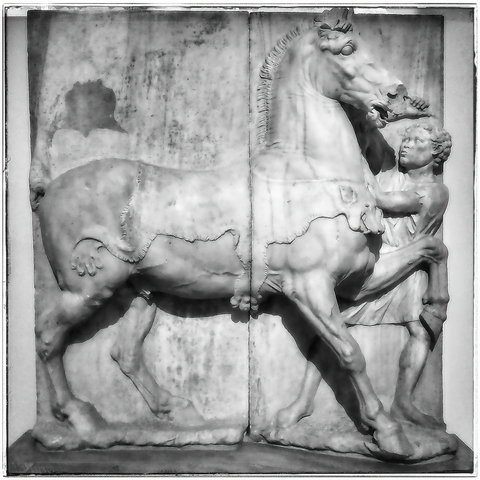
\includegraphics{smallthumb-lesson_I.jpeg}
\setfloatalignment{b}
\end{marginfigure}

\begin{abstract}
\noindent
Queste lezioni si articolano in \textsc{elementi grammaticali}, 
espressi sommariamente, seguiti da \textsc{vocabolari} per il lessico di base 
e da \textsc{frasi da tradurre} dal greco e in greco. 
\
L'approccio è quello del testo-laboratorio di morfosintassi: 
si presenta punto per punto - riprendendone la numerazione - 
l'esposizione di Gleason\cite{gleason1903}.\\
\bigskip
\noindent
Lezione I: qualche nozione generale sul sistema dei verbi del greco antico, 
il presente indicativo dei verbi in -ω, 
le desinenze personali dei tempi primari,
il primo vocabolario, esercizi.
\end{abstract}

%\printclassoptions

\newthought{38. Diatesi.} Il verbo greco ha tre diatesi: attiva, media e passiva.
L'attiva e la passiva sono come in latino (o in italiano); 
la diatesi media indica che il soggetto agisce su se stesso 
o a proprio vantaggio\sidenote{3 diatesi.}.

\newthought{39. Modo.} Ci sono quattro modi finiti o propri: 
indicativo, congiuntivo, ottativo e imperativo. 
Ci sono anche infiniti e participi, come in latino, 
e aggettivi verbali in \textbf{-τος} e \textbf{-τέος} 
\sidenote{4 modi finiti, 2 forme nominali.}.

\newthought{40. Tempo.} Ci sono sette tempi: presente, futuro, perfetto, 
futuro perfetto, imperfetto, aoristo, piuccheperfetto. 
I primi quattro sono detti \textsc{tempi primari} 
gli altri \textsc{tempi secondari} 
\sidenote{7 tempi: 4 primari, 3 secondari. 
Non tutti i tempi si coniugano in tutti i modi.}.

\newthought{41.} L' \textsc{Aoristo} indicativo corrisponde al perfetto storico 
latino, come in \textbf{ἔλυσε}, \textit{egli sciolse}; 
il perfetto al passato prossimo italiano, o al perfetto definito latino, 
come in \textbf{λέλυκε}, \textit{egli ha sciolto}.

\newthought{42. Numero.} Ci sono tre numeri: singolare e plurale, 
come in latino, e il duale, che indica due oggetti
\sidenote{3 numeri. Dal momento che il duale è raro, le relative flessioni sono riportate nelle sole tavole in appendice.}.

\newthought{43. Persona.} Ci sono tre persone, come in latino.

\newthought{44.} \textbf{I verbi hanno accento regressivo} (vedi 32.-34.)
\sidenote{se la desinenza si accorcia - rispetto a quella della persona precedente - allora l'accento torna sulla sillaba prima.}.

\newpage

\newthought{45. Il Presente Indicativo Attivo}

\begin{fullwidth}
\begin{table}[!htbp]
  \centering
  \begin{tabular}{l l l l l l l}
    %\toprule
	\multicolumn{7}{c}{\textsc{coniugazione del presente indicativo attivo}} \\
	 & \multicolumn{3}{c}{\textbf{λύω}, \textit{sciogliere, distruggere}} & \multicolumn{3}{c}{\textbf{ἄγω}, \textit{condurre, portare}} \\
    %\midrule
	& \multicolumn{6}{c}{\textsc{singolare}} \\
    \textsc{1.} & \textbf{λύ-ω}   & lu-o  & \textit{io sciolgo}    & \textbf{ἄγ-ω}   & ag-o  & \textit{io conduco}  \\
    \textsc{2.} & \textbf{λύ-εις} & lu-is & \textit{tu sciogli}    & \textbf{ἄγ-εις} & ag-is & \textit{tu conduci}  \\
    \textsc{3.} & \textbf{λύ-ει}  & lu-it & \textit{egli scioglie} & \textbf{ἄγ-ει}  & ag-it & \textit{egli conduce}  \\
	 & \multicolumn{6}{c}{\textsc{plurale}} \\
	\textsc{1.} & \textbf{λύ-ομεν} & lu-imus & \textit{noi sciogliamo} & \textbf{ἄγ-ομεν} & ag-imus & \textit{noi conduciamo}  \\
    \textsc{2.} & \textbf{λύ-ετε}  & lu-itis & \textit{voi sciogliete} & \textbf{ἄγ-ετε}  & ag-itis & \textit{voi conducete}  \\
    \textsc{3.} & \textbf{λύ-ουσι} & lu-unt & \textit{essi sciolgono} & \textbf{ἄγ-ουσι} & ag-unt & \textit{essi conducono}  \\
    %\bottomrule
  \end{tabular}
  \caption{λύω, ἄγω: presente indicativo attivo}
  \label{tab:normaltab}
  %\zsavepos{pos:normaltab}
\end{table}
\end{fullwidth}

\newthought{Osservazioni}
\begin{itemize}
\item[\textsc{1.}] La sillaba λύ- appare in tutte le flessioni. Questa è la \textit{radice verbale} o \textit{tema}.  
\item[\textsc{2.}] Confronta le terminazioni del verbo greco con quelle del latino \textit{luo, -is} e osserva le somiglianze.
\item[\textsc{3.}] Le terminazioni greche del presente (tempo primario) indicativo sono fatte dalla cosiddetta \textit{vocale variabile} \textbf{ο} o \textbf{ε} 
(che può essere indicata come \textbf{-ο/-ε}) e le \textit{desinenze personali (dei tempi primari)}

\begin{table}[!htbp]
  \centering
  \begin{tabular}{l c l}
    \textsc{singolare} & \hspace{10 mm} & \textsc{plurale} \\
    \textbf{[μι]} & \hspace{10 mm} & \textbf{μεν} \\
    \textbf{σ[ι]} & \hspace{10 mm} & \textbf{τε} \\
    \textbf{[τι(σι)]}  & \hspace{10 mm} & \textbf{(ν)σι}  \\
	
  \end{tabular}
  \caption{desinenze personali dei tempi primari}
  \label{tab:normaltab}
  %\zsavepos{pos:normaltab}
\end{table}
La vocale variabile è \textbf{ο} prima di \textbf{μ} ο \textbf{ν}, altrimenti è \textbf{ε}.

\end{itemize}

\newthought{46. Esercizio:} coniuga secondo lo schema il presente indicativo attivo dei seguenti verbi comuni:

\begin{table}[!htbp]
  \centering
  \begin{tabular}{l c l}
    
    \textbf{βάλλω,} \textit{getto, lancio} & \hspace{10 mm} & \textbf{μένω,} \textit{rimango} \\
    \textbf{γράφω,} \textit{scrivo} & \hspace{10 mm} & \textbf{πέμπω,} \textit{mando} \\
    \textbf{ἔχω,} \textit{ho, tengo} & \hspace{10 mm} & \textbf{φεύγω,} \textit{fuggo} \\
	
  \end{tabular}
  \caption{verbi comuni, presente indicativo attivo}
  \label{tab:normaltab}
  %\zsavepos{pos:normaltab}
\end{table}

\newthought{47. Leggi e traduci:}
\textsc{1.}~ἄγεις, βάλλει. \quad  
\textsc{2.}~φεύγομεν, ἔχετε. \quad
\textsc{3.}~ἄγουσι, πέμπω. \quad
\textsc{4.}~φεύγετε, γράφουσι. \quad
\textsc{5.}~βάλλεις, ἔχομεν. \quad
\textsc{6.}~ἔχεις, πέμπουσι. \quad
\textsc{7.}~γράφετε, μένει. \quad
\textsc{8.}~λύει, ἔχει, ἄγεις.


\newthought{48. Scrivi in greco, con accento e spirito:} 
\textsc{1.}~Egli manda, essi mandano. \quad  
\textsc{2.}~Tu scrivi, noi fuggiamo. \quad
\textsc{3.}~Voi portate, io ho. \quad
\textsc{4.}~Noi sciogliamo, tu sciogli.

\begin{figure*}[!b]
  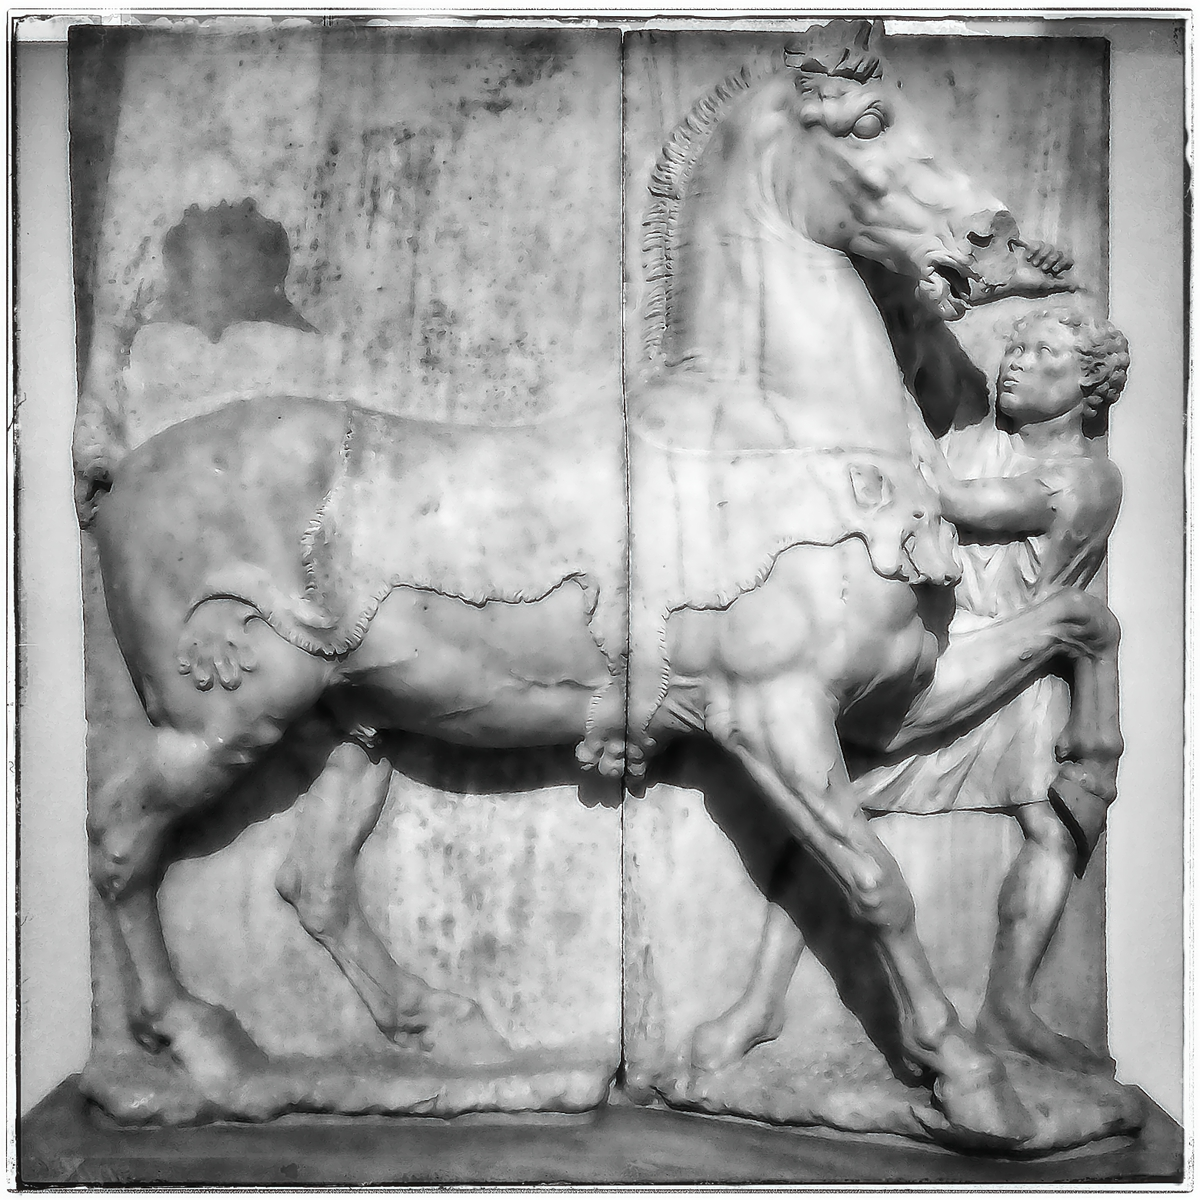
\includegraphics{thumb-lesson_I.jpeg}
  \caption{Museo Nazionale di Archeologia di Atene}
  \label{fig:textfig}
  %\zsavepos{pos:textfig}
  %\setfloatalignment{b}
\end{figure*}

\nobibliography{greekBiblio}
\bibliographystyle{alpha}


\end{document}
